\documentclass[11pt]{article}

% DeepMind-style preprint look built from standard packages.
\usepackage[a4paper,margin=1.05in,top=1.15in,headheight=14pt]{geometry}
\usepackage{amsmath,amssymb}
\usepackage{graphicx}
\usepackage{booktabs}
\usepackage{multirow}
\usepackage[dvipsnames]{xcolor}
\definecolor{dmblue}{RGB}{0,82,155}
\usepackage{tikz}
\usetikzlibrary{arrows.meta,positioning}
\usepackage{titlesec}
\usepackage[affil-it]{authblk}
\usepackage{natbib}
\usepackage{fancyhdr}
\usepackage{caption}
\usepackage[colorlinks=true,allcolors=dmblue]{hyperref}

\titleformat{\section}{\Large\sffamily\bfseries\color{dmblue}}{\thesection.}{0.6em}{}
\titleformat{\subsection}{\normalsize\sffamily\bfseries\color{dmblue}}{\thesubsection.}{0.6em}{}
\titleformat{\paragraph}[runin]{\sffamily\bfseries}{}{0em}{}[.]
\captionsetup{font=small,labelfont={bf,color=dmblue}}
\setlength{\parskip}{2pt}

\pagestyle{fancy}
\fancyhf{}
\fancyhead[L]{\small\sffamily\color{gray}Causal advisors vs.\ A/B tests for subscription decisions}
\fancyhead[R]{\small\sffamily\thepage}
\renewcommand{\headrulewidth}{0pt}
\fancyfoot[L]{\footnotesize\sffamily\color{gray}Preprint. All results come from a simulation. See the Limitations section.}

\title{\sffamily\bfseries\boldmath\color{dmblue}
When Should a Subscription Business Trust Causal Inference Instead of an A/B Test?\\
\large\normalfont\sffamily\color{black}A simulation study of paywall and pricing decisions}
\author{Vasanth Pugalenthi\thanks{Corresponding author: \texttt{vasanth.pugalen@gmail.com}}}
\affil{Subscription-Causal-Inference project}
\date{October 9, 2026}

\begin{document}
\maketitle
\thispagestyle{fancy}

\begin{abstract}
\noindent
Subscription businesses decide what to paywall and what to charge using
dashboard comparisons, and sometimes A/B tests. We compare both against a
causal advisor: a method that estimates the effect of a change from the
company's own historical data, corrects for the biases it can see, and asks
for an experiment when the data cannot support a conclusion. We score all
three inside a simulated subscription business where the true effect of every
change is known, measuring the profit each method's decisions lose. Each
incumbent has a situation that ruins it. The dashboard fails when the right
move looks wrong on the surface. The short A/B test fails when the damage
arrives more slowly than the test: it approves a harmful paywall in 97
percent of those runs, losing \$5{,}380 per thousand users per year, worse
than doing no analysis at all. The advisor is never the worst method in any
situation and correctly asks for an experiment when history contains no
signal. Its value is not accuracy against a good test. It is avoiding the big
mistakes, and knowing when a test is truly needed.
\end{abstract}

\section{Introduction}
A software product with a free tier and a paid tier faces two recurring
questions. If we lock feature X behind the paid tier, do we gain upgrades or
just lose users? If we raise the price 20 percent, does revenue go up or
down? The usual answers come from a dashboard: ``users of feature X upgrade
three times more often'' or ``conversion did not drop after our last price
increase.'' Both readings are confounded. Engaged users upgrade more whether
or not the feature causes it, and businesses raise prices when things are
already going well, so the change gets credit for growth it did not create.
The textbook fix, a randomized test, is often impractical: price tests upset
customers, and retention effects need months to show up, so a short test can
look clean and still point the wrong way.

This paper studies a middle path, a \emph{causal advisor}
(Figure~\ref{fig:flow}). It uses the data the company already has, adjusts
for differences it can measure, and stress tests the answer against what it
cannot. If the decision survives, it recommends an action; if not, it asks
for a specific experiment. The design follows \citet{cadahia2026}, who built
a similar gate for retail pricing. Our question: does this policy beat the
two things businesses actually do?

Real data cannot answer that, because it never shows what the other choice
would have done. Following the logic of the ACIC benchmarks \citep{hahn2019},
we build a simulation where the truth is known and score every method on
profit lost, over 30 repetitions of every setting.

\begin{figure}[t]
\centering
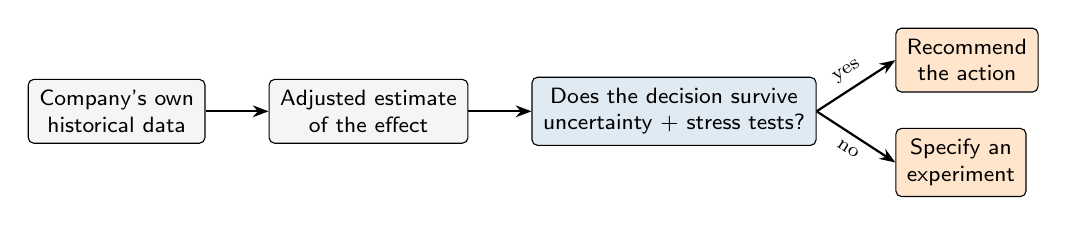
\begin{tikzpicture}[
  font=\footnotesize\sffamily,
  box/.style={draw, rounded corners=2pt, align=center, inner sep=4pt,
              minimum height=8mm, fill=gray!8},
  dec/.style={draw, rounded corners=2pt, align=center, inner sep=4pt,
              minimum height=8mm, fill=dmblue!12},
  act/.style={draw, rounded corners=2pt, align=center, inner sep=4pt,
              minimum height=8mm, fill=orange!20},
  arr/.style={-{Stealth[length=2mm]}, thick}]
\node[box] (data) {Company's own\\historical data};
\node[box, right=8mm of data] (est) {Adjusted estimate\\of the effect};
\node[dec, right=8mm of est] (gate) {Does the decision survive\\uncertainty + stress tests?};
\node[act, right=10mm of gate, yshift=6.5mm] (go) {Recommend\\the action};
\node[act, right=10mm of gate, yshift=-6.5mm] (exp) {Specify an\\experiment};
\draw[arr] (data) -- (est);
\draw[arr] (est) -- (gate);
\draw[arr] (gate.east) -- node[above, sloped, font=\scriptsize]{yes} (go.west);
\draw[arr] (gate.east) -- node[below, sloped, font=\scriptsize]{no} (exp.west);
\end{tikzpicture}
\caption{\textbf{The causal advisor.} It acts only when the recommendation
survives both statistical uncertainty and a stress test for hidden bias;
otherwise it outputs a concrete experiment request.}
\label{fig:flow}
\end{figure}

\section{The simulated business}
We simulate a freemium product month by month over one year: free users
bring in \$2 per month from ads, the paid tier costs \$10 per month. Each
user has an engagement level, a willingness to pay, and a hidden taste
factor no method ever observes. Engaged users use more, stay longer, and
upgrade more. Because we control the simulation, we can replay the same
world under both choices and read off the true profit difference. The
methods see only what a real company would: noisy user attributes, feature
usage, upgrades, cancellations, revenue.

\paragraph{Decision one: lock a feature behind the paywall} Feature X is
free today, and heavier users adopt it more, so adopters look great on any
dashboard even when the feature does little. A hidden-bias dial controls how
strongly the unobserved taste factor also drives adoption. Locking cuts both
ways: some users pay to unlock, others get frustrated and quit over the
following months. We run two worlds: one where the feature is mildly useful
and locking earns about \$2.70 per user per year, one where it is a core
reason people stay and locking loses about \$5.50. The dashboard reads
almost the same in both.

\paragraph{Decision two: raise the price 20 percent} The business has three
years of signup history and considers moving from \$10 to \$12. In some runs
it raised the price once before, right when the product was improving, which
poisons before/after comparisons; in others the price never changed, so
history says nothing about price sensitivity. Demand is either insensitive
(the raise earns) or sensitive (the raise loses).

\paragraph{Scoring} Each method picks an action. Its \emph{regret} is the
profit given up by choosing wrong, plus any real testing costs it chose to
pay (test users on the worse option, waiting for results), in dollars per
thousand users per year.

\section{The three methods}
All three feed their estimate into the same simple profit formula; they
differ only in evidence quality and willingness to say ``not yet.''
\textbf{Dashboard}: compare adopters with non-adopters; for pricing, compare
conversion before and after the old change, and if price never changed,
assume demand will not react. \textbf{Causal advisor}: compare adopters with
statistically similar non-adopters; for pricing, fit a demand model
controlling for trend and seasonality. Then stress test: widen the
uncertainty range and re-estimate as if the most important attribute were
missing; if the decision flips anywhere in that range, request an experiment
instead of acting. \textbf{A/B test}: a randomized test as a busy company
runs one, 10 percent of users for three months (paywall) or two months
(pricing), short-term result scaled to a year. The randomization is honest;
the scaling is the risk.

\begin{figure}[t]
  \centering
  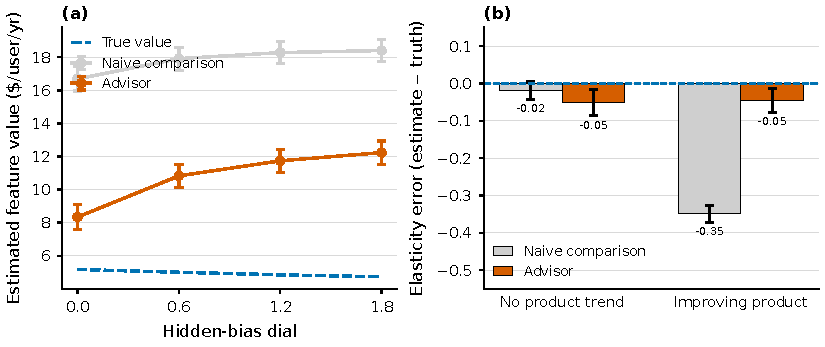
\includegraphics[width=0.92\linewidth]{figs/estimates-vs-truth.pdf}
  \caption{\textbf{Why the dashboard gets fooled, and how much the advisor
  fixes.} \textbf{(a)}~Paywall: estimated dollar value of the feature vs.\
  the hidden-bias dial (mean over both worlds, 95 percent intervals, 30
  repetitions). The dashboard reads \$17--18 when the truth is about \$5;
  the advisor removes most, not all, of the gap. \textbf{(b)}~Pricing: error
  in estimated price sensitivity when the past change coincided with an
  improving product. Before/after is off by $-0.35$; the trend-controlled
  advisor stays near zero.}
  \label{fig:bias}
\end{figure}

\begin{figure}[t]
  \centering
  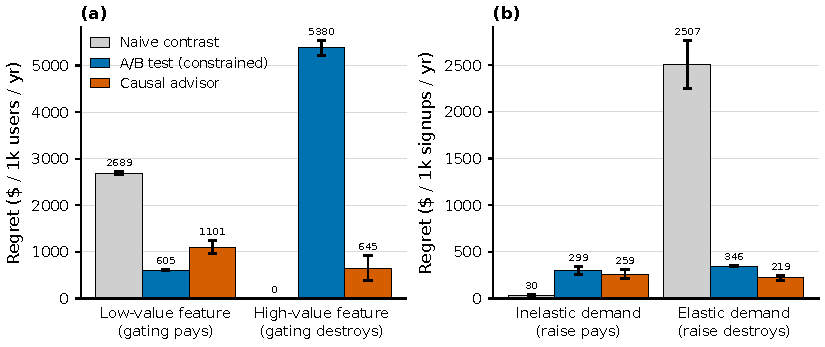
\includegraphics[width=0.92\linewidth]{figs/regret-by-regime.pdf}
  \caption{\textbf{Every method except the advisor has a situation that
  ruins it.} Profit lost per thousand users per year (95 percent intervals,
  30 repetitions). \textbf{(a)}~Paywall: the dashboard never locks, missing
  the profitable paywall; the three month A/B test misses slow churn damage
  and approves the harmful one. \textbf{(b)}~Pricing: the dashboard raises
  into price-sensitive demand; the A/B test does well because pricing
  feedback is fast.}
  \label{fig:regret}
\end{figure}

\section{Results}

\begin{table}[t]
\centering
\caption{\textbf{Overall scores.} Accuracy is the share of runs choosing the
truly better action; regret is average profit lost per thousand users
(paywall) or signups (pricing) per year; the last column is how often the
advisor asked for an experiment. Per-situation breakdowns in
Figure~\ref{fig:regret}.}
\label{tab:overall}
\small
\begin{tabular}{llrrr}
\toprule
Decision & Method & Accuracy & Regret (\$/1k/yr) & Asked for test \\
\midrule
\multirow{3}{*}{Paywall}
 & dashboard & 0.50 & 1{,}345 & \\
 & A/B test  & 0.51 & 2{,}992 & \\
 & advisor   & \textbf{0.83} & \textbf{873} & 44\% \\
\midrule
\multirow{3}{*}{Pricing}
 & dashboard & 0.68 & 1{,}268 & \\
 & A/B test  & 0.88 & 323 & \\
 & advisor   & \textbf{0.90} & \textbf{239} & 72\% \\
\bottomrule
\end{tabular}
\end{table}

\paragraph{The dashboard fails when the right move looks wrong}
Figure~\ref{fig:bias}a shows the mechanism: the raw adopter comparison
overrates the feature by roughly a factor of three at every level of the
hidden-bias dial. Convinced the feature is precious, the dashboard never
locks it, which is exactly wrong in the world where locking pays (\$2{,}689
lost per thousand users per year, Figure~\ref{fig:regret}a). In pricing, the
misread elasticity (Figure~\ref{fig:bias}b) plus the ``demand won't react''
default make it raise into sensitive demand, losing up to \$5{,}446 per
thousand signups. The failure is systematic: the same confident reading
appears in worlds that need opposite answers.

\paragraph{The A/B test fails when damage is slower than the test}
In the three month paywall test, unlock revenue arrives quickly but
frustration churn has barely started. Scaled to a year, the early revenue
wins, and the test approves the harmful paywall in 97 percent of those runs,
losing \$5{,}380 per thousand users per year, worse than no analysis at all.
The pricing test is fine because conversion reacts within the window
(Figure~\ref{fig:regret}b). A short test is a bet that the effects you care
about arrive quickly.

\paragraph{The advisor is never the worst option}
Its adjustment removes about half the bias (Figure~\ref{fig:bias}), enough
to choose correctly most of the time, and its stress test converts many
remaining dangerous calls into ``run an experiment,'' including every run
where the price had never changed. It posts the lowest overall regret in
both decisions (Table~\ref{tab:overall}), and its worst situation
(\$1{,}101) is far safer than the dashboard's (\$2{,}689) or the A/B test's
(\$5{,}380). One surprise: when the advisor declines the paywall question it
hands the decision to the A/B test, which is usually wrong in the world
where locking backfires, so the advisor inherits part of that error. Asking
for a test is only as safe as the test; the advisor must also specify how
long to run it and what to measure.

\section{Limitations and conclusion}
These numbers show a pattern, not what any real company would measure. We
tuned both the simulator and the methods, with no separation between test
maker and test taker \citep{hahn2019}; the A/B failure follows from the
short window and crude scale-up we gave it, and a longer test or better
early indicators would close much of that gap; all methods share one
simplified profit formula; and the advisor's stress test is a heuristic
stand-in for formal sensitivity analysis \citep{chernozhukov2018}, which
matters because even careful adjustment can miss, as paired experimental and
observational data at Microsoft recently showed \citep{young2026}.
Semi-synthetic replication on real subscription data is the next step.

The conclusion the study supports: the two methods businesses actually use
are gambles on which world they live in, each disastrous in a situation the
other survives. The causal advisor, which adjusts for what it can measure
and asks for an experiment when the answer is not solid, was never the worst
option. That is the honest pitch: not ``better than an A/B test,'' but
``never the method that quietly loses five dollars per user per year.''

\begin{thebibliography}{6}

\bibitem[Cadahia Delgado(2026)]{cadahia2026}
P.~Cadahia Delgado.
\newblock ACT, WAIT, or EXPERIMENT: A causal governance framework for retail
  price optimization under abstentions.
\newblock arXiv:2609.10615, 2026.

\bibitem[Chernozhukov et al.(2018)]{chernozhukov2018}
V.~Chernozhukov, D.~Chetverikov, M.~Demirer, E.~Duflo, C.~Hansen, W.~Newey,
  and J.~Robins.
\newblock Double/debiased machine learning for treatment and structural
  parameters.
\newblock \emph{The Econometrics Journal}, 21(1):C1--C68, 2018.

\bibitem[Hahn et al.(2019)]{hahn2019}
P.~R. Hahn, V.~Dorie, and J.~S. Murray.
\newblock Atlantic Causal Inference Conference (ACIC) data analysis
  challenge 2017.
\newblock arXiv:1905.09515, 2019.

\bibitem[LaLonde(1986)]{lalonde1986}
R.~J. LaLonde.
\newblock Evaluating the econometric evaluations of training programs with
  experimental data.
\newblock \emph{American Economic Review}, 76(4):604--620, 1986.

\bibitem[Young et al.(2026)]{young2026}
J.~Young, M.~Ngatia, and E.~W. Dillon.
\newblock Reevaluating causal estimation methods with data from a product
  release.
\newblock arXiv:2601.11845, 2026.

\end{thebibliography}

\appendix
\section{Reproducibility, compute, and disclosure}
The simulator, methods, and scoring code live in the project repository.
Each experiment is a frozen branch answered by one logged run (IDs
\texttt{9e9cde5b} and \texttt{06bd0de4}). Runs are seeded, and true effects
come from replaying identical random draws under both choices. Everything
runs on an ordinary CPU in under five minutes, in a Python environment with
NumPy as the only dependency, rebuilt by the fixed command \texttt{bash
run.sh}. This paper was drafted by an LLM research agent (Claude, Anthropic)
operating the simulator and literature tools, with the human author
directing the question, scope, and revisions. All reported numbers are read
from logged runs.

\end{document}
